\documentclass[aspectratio=169]{beamer}
\graphicspath{ {./images/}}
\usepackage{setspace}
\usepackage{hyperref}

\title{CP Rate My Professor}
\author[CP Rate My Professor Team]{Naphat Darunaitorn\\ Noppakorn Jiravaranun\\ Nopparuj Poonsubanan\\ Ittipat Yodprasit}
\usetheme[]{Berlin}
\setbeamertemplate{navigation symbols}{}
\makeatletter
  \setbeamertemplate{footline}{%
    \begin{beamercolorbox}[colsep=1.5pt]{upper separation line foot}
    \end{beamercolorbox}
    \begin{beamercolorbox}[ht=2.5ex,dp=1.125ex,%
      leftskip=.3cm,rightskip=.3cm plus1fil]{author in head/foot}%
      \leavevmode{\usebeamerfont{author in head/foot}\insertshortauthor}%
      \hfill%
      {\usebeamerfont{institute in head/foot}\usebeamercolor[fg]{institute in head/foot}\insertshortinstitute}%
    \end{beamercolorbox}%
    \begin{beamercolorbox}[ht=2.5ex,dp=1.125ex,%
      leftskip=.3cm,rightskip=.3cm plus1fil]{title in head/foot}%
      {\usebeamerfont{title in head/foot}\insertshorttitle\hfill\insertframenumber}%
    \end{beamercolorbox}%
    \begin{beamercolorbox}[colsep=1.5pt]{lower separation line foot}
    \end{beamercolorbox}
  }
\makeatletter

\begin{document}
\frame{\titlepage}
\section{Introduction}
\begin{frame}
    \frametitle{Online Learning}
    \centering
    
\includegraphics[scale=0.5]{online_learning.jpg}
\end{frame}
\begin{frame}
    \centering
    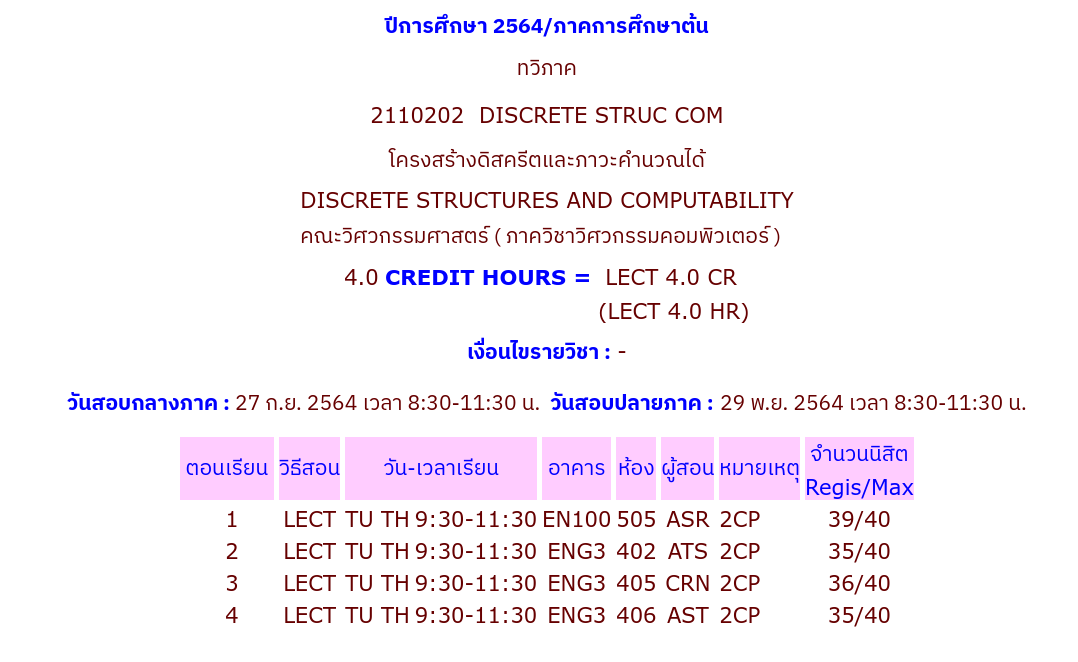
\includegraphics[scale=0.4]{discrete_section.png}
\end{frame}
\begin{frame}
    \frametitle{A sad, true story}
    \pause
    \begin{columns}
        \begin{column}{0.4\textwidth}
            \centering
            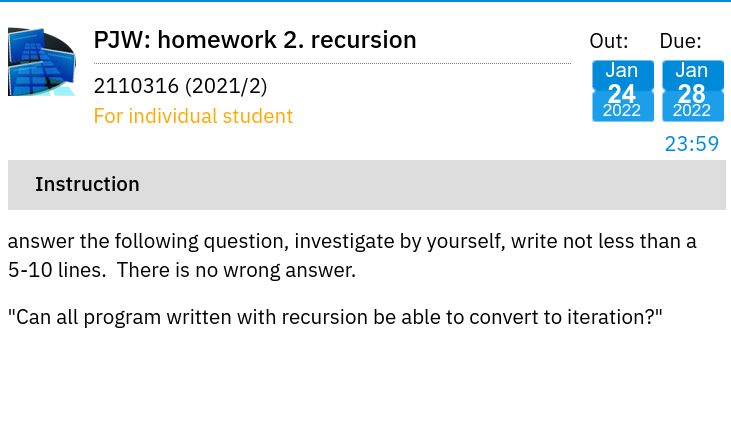
\includegraphics[scale=0.3]{proglangsec1}
            
\includegraphics[scale=0.5]{proglangsec1_nowrong}
        \end{column}
        \pause
        \begin{column}{0.4\textwidth}
            \centering
            
\includegraphics[scale=0.2]{proglangsec2}
        \end{column}
    \end{columns}
    \begin{flushright}
        \tiny{Meme from: \textbf{CP47 High //Quality Meme}}
    \end{flushright}
\end{frame}

\begin{frame}
    \frametitle{Existing Solution}
    \begin{columns}
        \begin{column}{0.5\textwidth}
            \begin{itemize}
                \item CU-CAS?
                      \begin{itemize}
                          \item {\color{red}Not anonymous}
                          \item {No useful information for students}
                          \item {The rating system is arbitrary}
                      \end{itemize}
            \end{itemize}
        \end{column}
        \begin{column}{0.5\textwidth}
            \centering
            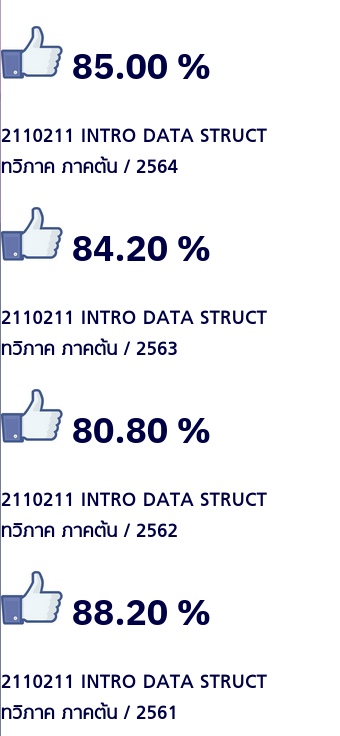
\includegraphics[scale=0.3]{cucas_score.png}
        \end{column}
    \end{columns}
\end{frame}
\section{Application}
\begin{frame}
    \centering
    \begin{spacing}{3}
        {\huge \textbf{Meet} }\pause\\
        {\huge \color{cyan}\textbf{CP Rate My Professor}}
    \end{spacing}
\end{frame}
\begin{frame}
    \frametitle{CP Rate My Professor}
    \begin{itemize}
        \item CP Rate My Professor is a platform for commenting and rating professor
        \item Help with answering the question of\pause
              \begin{spacing}{1.25}
                  \begin{itemize}
                      \item How do I prepare for this course?\pause
                      \item Which course should I take?\pause
                      \item Which section to choose?\pause
                      \item Which professor I should do INDIV with?
                  \end{itemize}
              \end{spacing}
    \end{itemize}
\end{frame}
\begin{frame}
    \frametitle{Home Page}
    \centering
    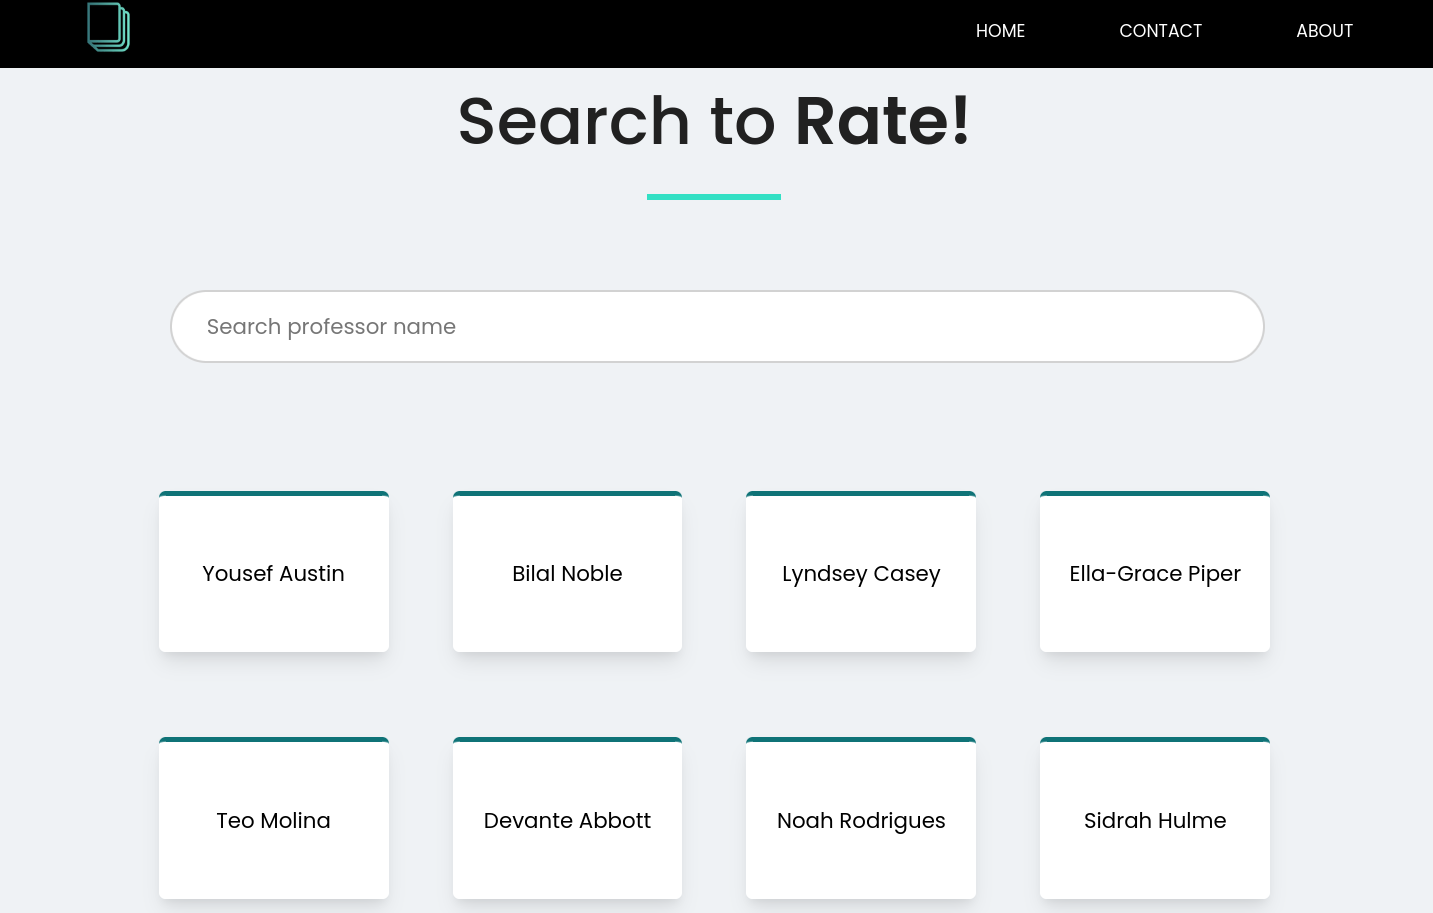
\includegraphics[scale=0.25]{ratemyprof_home.png}
\end{frame}
\begin{frame}
    \frametitle{Professor Page}
    \centering
    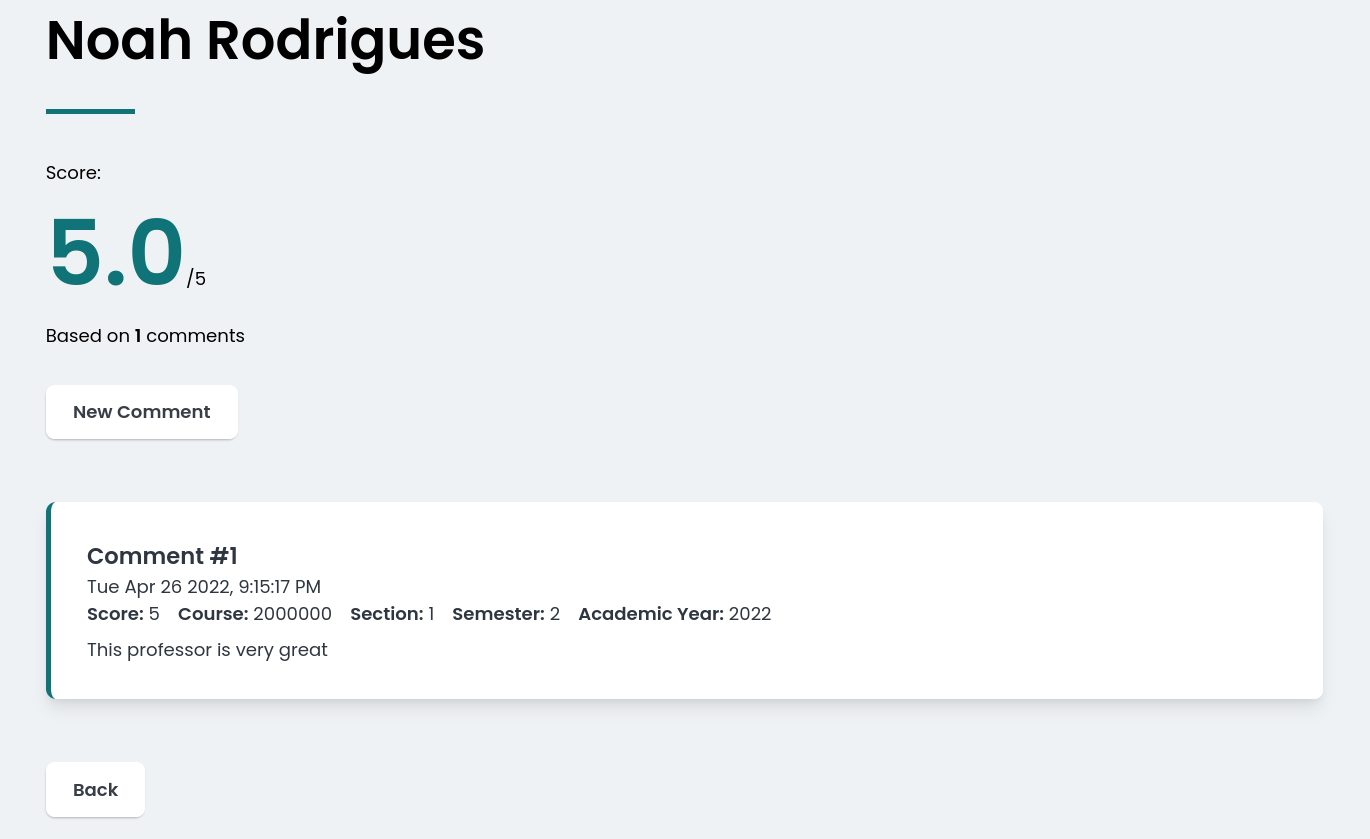
\includegraphics[scale=0.25]{ratemyprof_prof.png}
\end{frame}
\begin{frame}
    \frametitle{New Comment Page}
    \centering
    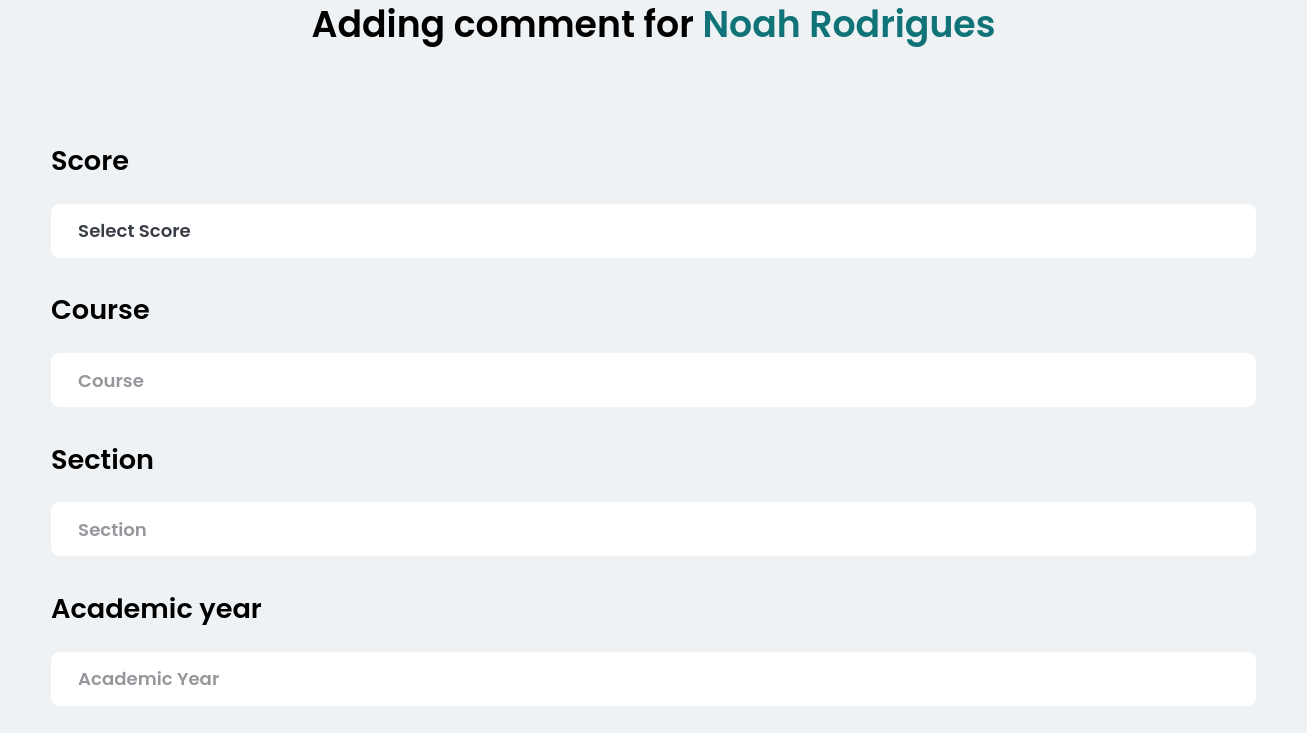
\includegraphics[scale=0.25]{ratemyprof_comment.png}
\end{frame}
\section{Demonstration}
\begin{frame}
    \frametitle{Demonstration}
    \centering
    {\huge\textbf{Let's see the site}}\\~\\
    See the site together with us at \\
    {\color{blue}\url{https://cp-rate-my-professor.web.app}}
\end{frame}
\section{Goals}
\begin{frame}
    \frametitle{Goals}
    \begin{spacing}{1.5}
        \begin{itemize}
            \item {\color{blue}\textbf{Transparency}} and {\color{blue}\textbf{Anonymity}}
                  \begin{itemize}
                      \item We do not track our users
                      \item We only keep information that is in the comment only
                      \item User does \textbf{not} require to login to make a comment
                  \end{itemize}
            \item Be a safe space for giving comments and ratings
        \end{itemize}
    \end{spacing}
\end{frame}
\begin{frame}
    \frametitle{Important details when using the application}
    \begin{itemize}
        \item We do not allow the deletion of comment
        \item Contact us at contact page
        \item If we have information that can be proven to be false we will put the information with the comment
    \end{itemize}
\end{frame}
{
\setbeamertemplate{headline}{}
\begin{frame}
    \centering
    \huge{\textbf{Thank You!}}
\end{frame}
\end{document}
}